\documentclass[11pt,a4paper]{article}

% ══════════════════════════════════════════════════════════════
% Packages
% ══════════════════════════════════════════════════════════════
\usepackage[T1]{fontenc}
\usepackage{lmodern}
\usepackage[margin=1in]{geometry}
\usepackage{amsmath,amssymb}
\usepackage{graphicx}
\usepackage{booktabs}
\usepackage{xcolor}
\usepackage{hyperref}
\usepackage{caption}
\usepackage{enumitem}
\usepackage{authblk}
\usepackage{tabularx}
\usepackage{float}
\usepackage{fancyvrb}
\usepackage{microtype}

\graphicspath{{../figures/}}

% Absorb long URLs cleanly
\setlength{\emergencystretch}{3em}
\hyphenpenalty=1500
\exhyphenpenalty=100

\hypersetup{
  colorlinks=true,
  linkcolor=blue!70!black,
  citecolor=green!50!black,
  urlcolor=blue!60!black,
}

\captionsetup{font=small,labelfont=bf}

\newcommand{\code}[1]{\texttt{#1}}

% ══════════════════════════════════════════════════════════════
% Title
% ══════════════════════════════════════════════════════════════
\title{%
  \textbf{Fugue}: Score-Conditioned Music Covers\\
  by Grafting Frozen Generators%
}

\author[1]{Jing Zhang\thanks{Code, samples, and evaluation records: \url{https://github.com/HenryZ838978/fugue}}}
\affil[1]{Independent Research}

\date{September 2026}

\begin{document}

\maketitle

% ══════════════════════════════════════════════════════════════
\begin{abstract}
\noindent
A useful music cover must remain recognizable as the source song while adopting a different arrangement and production style. Fugue combines YuE2-3B's score-conditioned generation with MiniMax-Music3's diffusion-based acoustic renderer, without updating either pretrained model. A 66.6M-parameter adapter maps YuE2's acoustic latents into the renderer's existing conditioning interface. The adapter requires no additional original/cover pairs or human annotations: its inputs and targets are constructed from the audio and stored codes of MM3's own generations. On 209 real songs covered into two target styles each, the current version, Fugue v4, achieves source-song retrieval MRR 0.609 versus 0.646 for YuE2's native decoder; a style-only control yields 0.022. Across the same 418 generated latents, median spectral rolloff rises from 13.8 to 17.6~kHz and stereo side/mid power from $-10.9$ to $-4.8$~dB. These measurements describe increased high-frequency content and a wider stereo image from MM3's pretrained DiT-based rendering path, rather than an overall quality ranking. We release the adapter, inference package, resident services, cover frontend, evaluation records, and figure-generation code. Fugue provides a practical alternative for score-conditioned covers by combining a learned cross-model interface with end-to-end deployment and evaluation infrastructure.
\end{abstract}

% ══════════════════════════════════════════════════════════════
\section{Introduction}
% ══════════════════════════════════════════════════════════════

Cover generation starts from musical material that a user already wants to keep. The task is to change its setting: for example, turn a vocal recording into a piano arrangement, or realize the same song as guitar-driven rock. This makes identity preservation, style control, and acoustic rendering jointly important. A convincing output in the requested genre is not a successful cover if it has lost the intended song.

YuE2-3B~\cite{yue2} provides score-conditioned music generation, including ABC input and a non-autoregressive acoustic stage. MiniMax-Music3 (MM3)~\cite{mm3} supplies the pretrained diffusion transformer and stereo vocoder used for Fugue's acoustic rendering. We use the former to generate score-conditioned musical content and the latter to render it. The models are connected before waveform decoding through a learned latent mapping. The resulting system offers another route to music covers, with more high-frequency content and a wider stereo image than the native decoder in the paired evaluation.

\begin{figure}[t]
    \centering
    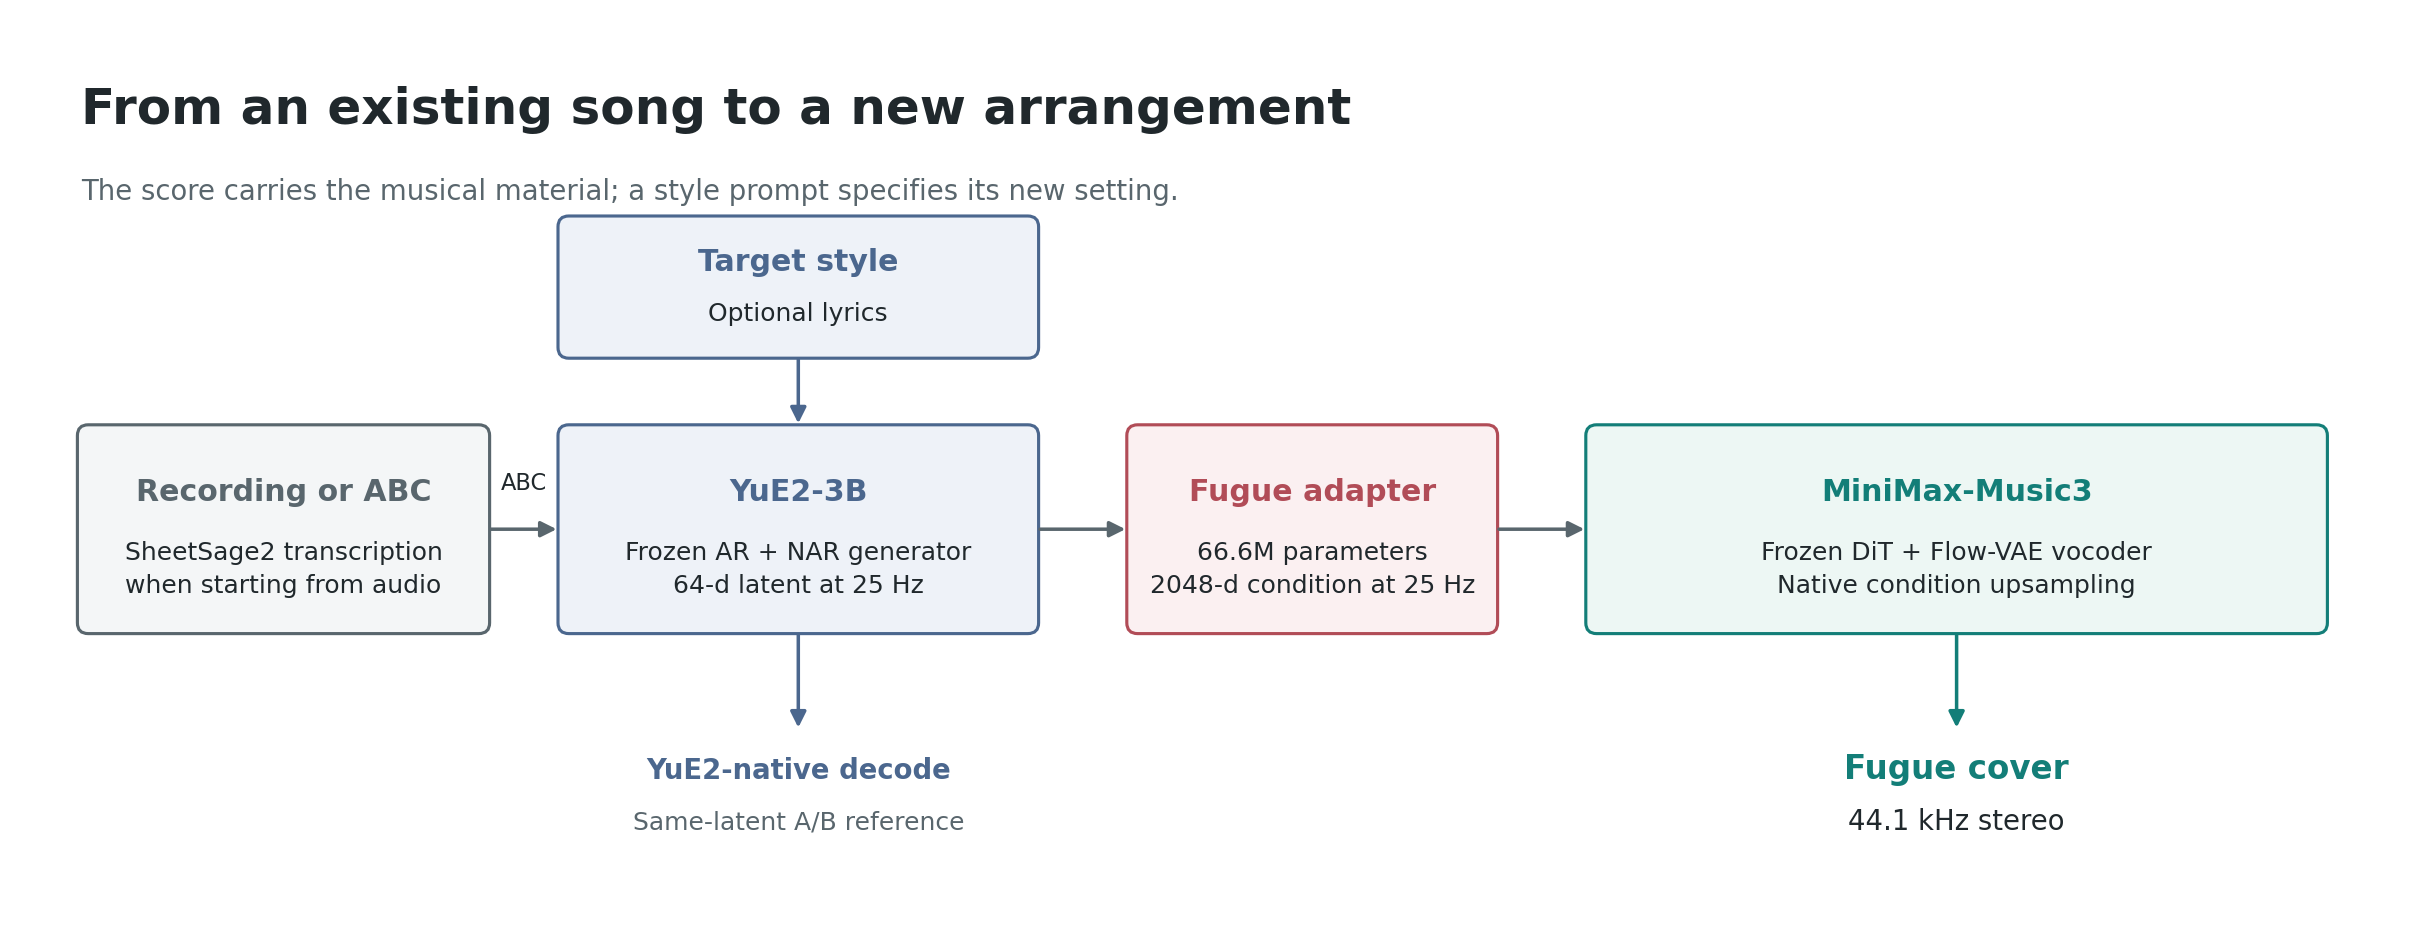
\includegraphics[width=0.96\linewidth]{cover-workflow.png}
    \caption{Fugue inference pipeline and its native-decoder reference branch. A recording is transcribed into ABC, or a score is supplied directly. YuE2 generates an acoustic latent under the score and style prompt. Fugue maps that latent into MM3's native DiT condition. The native YuE2 decoder provides a paired reference for isolating the rendering change.}
    \label{fig:workflow}
\end{figure}

The name \textbf{Fugue} draws on the return of a recognizable subject through interweaving musical voices. It expresses a design goal: keep continuity in a vocal or instrumental line while allowing its surroundings to change and respond. The current system realizes this through score-conditioned generation of mixed audio.

The central contribution is \textbf{a way to compose existing capabilities without additional cover-pair supervision}. Training examples are constructed from MM3 generations with stored RVQ codes; no recording has to be paired with a human or model-produced cover. We also identify a usable cross-model interface, correct the time-axis mismatch introduced by chunked rendering, and evaluate the resulting system on real-song covers. The main experiment appears in Section~\ref{sec:eval}; the unsuccessful attempts to train score conditioning directly into MM3 are retained in Appendix~\ref{app:direct}.

A second contribution is \textbf{the infrastructure that makes this composition usable and inspectable}: a training-pair extraction pipeline, a packaged adapter with normalization statistics, separate resident services that can share one GPU, a cover CLI and frontend, long-form chunked inference, and resumable paired evaluation. Section~\ref{sec:infra} describes these components and distinguishes Fugue's integration work from the capabilities inherited from the frozen models.

% ══════════════════════════════════════════════════════════════
\section{Method}
% ══════════════════════════════════════════════════════════════

\subsection{A shared interface for training and inference}

YuE2's AR path produces semantic tokens, and its NAR flow-matching stage produces an acoustic latent \code{z} with 64 dimensions at 25~Hz. The public YuE2 VAE encoder maps audio into the same latent format. We choose this representation because it is available both from training audio and from score-conditioned generation. YuE2's NAR hidden states vary with the denoising step; they are not the fixed interface used here.

MM3 normally constructs its DiT condition from hidden states of its language model and RVQ depth decoder. We target the 2048-dimensional output of \code{ConditionEncoder} \textbf{before temporal upsampling}, denoted \code{c25}. The adapter predicts \code{c25} from \code{z}; MM3's upsampling, DiT, and vocoder then run unchanged. YuE2's native VAE decoder and MM3's LM/depth decoder are not used on the main cover-generation path.

\begin{Verbatim}[frame=single,fontsize=\small,samepage=true,xleftmargin=1em,xrightmargin=1em]
z: (T, 64), 25 Hz
    -> Fugue adapter
    -> c25: (T, 2048), 25 Hz
    -> MM3 native nearest-neighbor upsampling
    -> frozen DiT and Flow-VAE vocoder
    -> 44.1 kHz stereo
\end{Verbatim}

The two representations have the same nominal frame rate. MM3's chunked rendering nevertheless introduces a time-axis drift that must be corrected when pairing the training data.

\subsection{Supervision from self-generated recordings}

The paired corpus contains 12,837 MM3 generations, approximately 191 hours, with audio, RVQ codes, captions, and lyrics. For each generation we construct:

\begin{enumerate}[leftmargin=2em,itemsep=0.2em]
    \item \textbf{Input:} resample the rendered audio from 44.1 to 48~kHz and encode it with the frozen YuE2 VAE encoder.
    \item \textbf{Target:} teacher-force the stored codes and original prompt through MM3's frozen LM and depth decoder, then apply \code{ConditionEncoder} through its projection layer to recover \code{c25}.
\end{enumerate}

\begin{figure}[t]
    \centering
    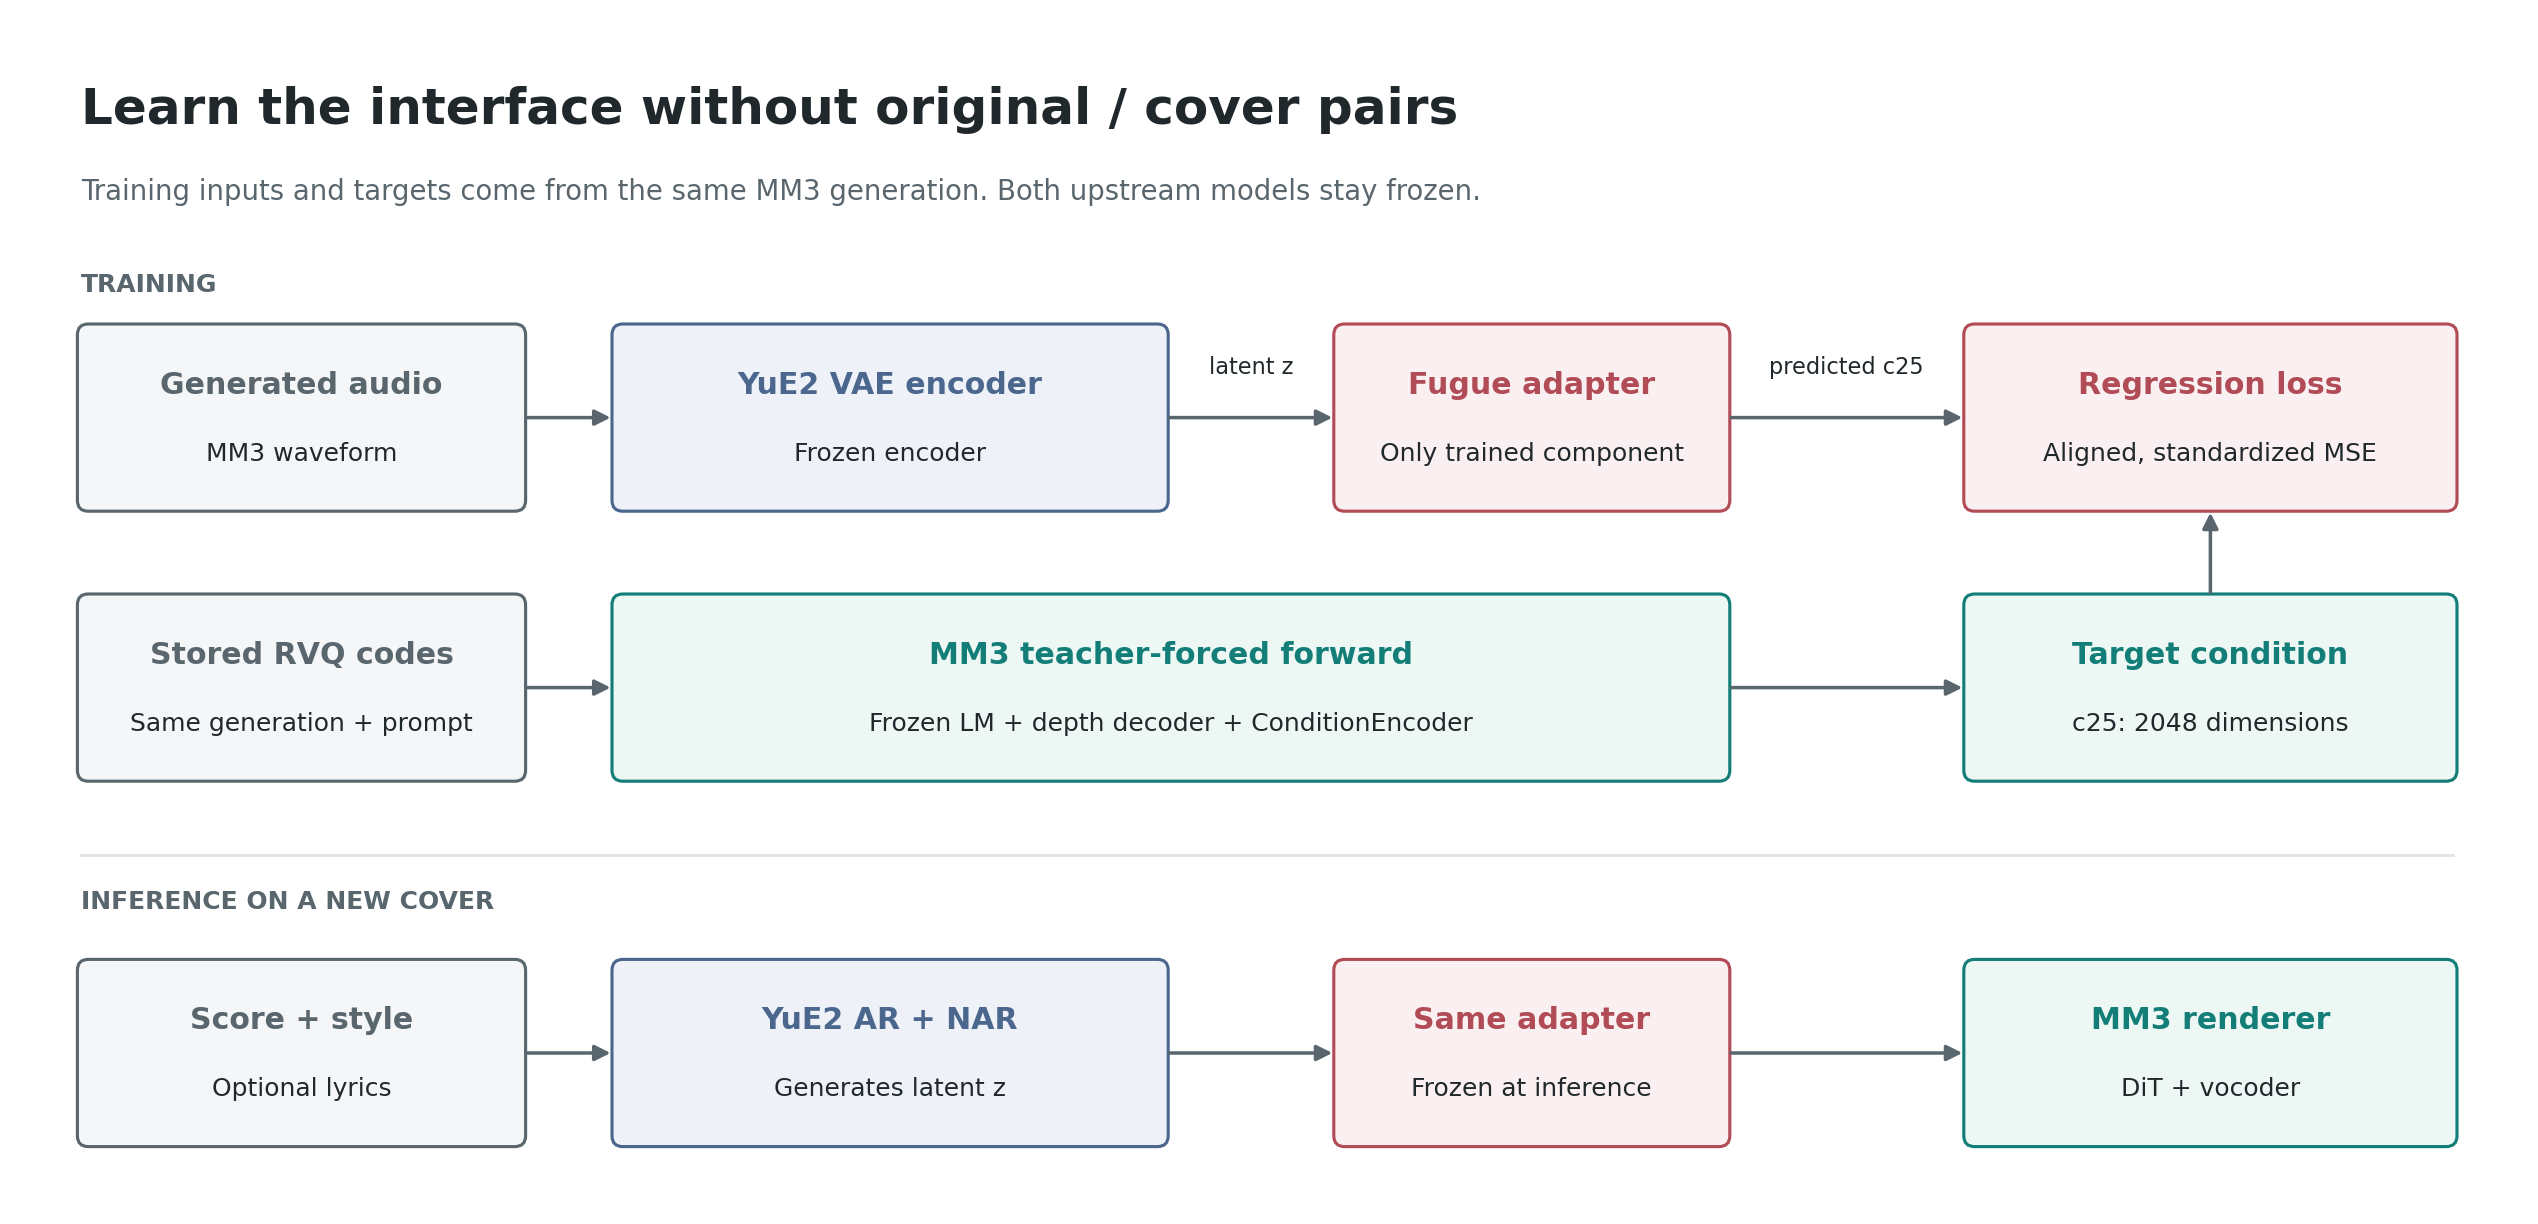
\includegraphics[width=0.96\linewidth]{training-pairs.png}
    \caption{Training and inference paths, highlighting the shared adapter and the construction of supervision from one MM3 generation. Both sides of a training pair describe the same generated recording. At inference, YuE2's score-conditioned AR/NAR generator replaces the VAE encoder as the source of \code{z}. Only the adapter is optimized. No original/cover pairs are used in this adaptation stage.}
    \label{fig:pairs}
\end{figure}

Stored generation codes avoid the need for MM3's unreleased audio-to-RVQ quantizer. In a reconstruction check, rendering the teacher-forced condition gives log-mel L1 0.686 to the stored original, compared with 0.698 between two renders using different DiT seeds. This provides an empirical consistency check on condition recovery.

Training uses encoder latents while cover inference uses NAR-generated latents. These inputs share a format but need not share a distribution. We therefore normalize channels and add Gaussian noise to the training inputs. Evaluation on real-song covers tests the complete path through transcription, YuE2 generation, and the adapter.

\paragraph{Temporal alignment.} MM3 renders 200-frame windows with a 100-frame hop. Each full window yields 689 acoustic latents; stitching advances 345 latents per hop instead of the nominal 344.53125. Consequently, frame $j$ of the MM3 condition corresponds approximately to YuE2 frame

\begin{Verbatim}[frame=single,fontsize=\small,samepage=true,xleftmargin=1em,xrightmargin=1em]
m(j) = round(j + 0.136054 * k(j))
k(j) = 0                              if j < 125
       floor((j - 25) / 100)           otherwise
\end{Verbatim}

The implementation clamps $k(j)$ to the final rendering window and clips the resulting input index. The coefficient is $345 / (441/128) - 100$. Accounting for this drift raises the three-frame-context ridge probe from $R^2$ 0.262 to 0.347 in the alignment experiment.

\subsection{Adapter and optimization}

The adapter consists of a 64-to-768 linear projection, two residual local convolutions of kernel size 5, a residual grouped positional convolution of kernel size 63 with 16 groups, eight pre-LN bidirectional Transformer layers with 12 heads, and a final normalization and 768-to-2048 projection. It has 66.6M parameters and no absolute position embeddings.

Inputs and targets are standardized per channel. Let \code{y\_tc} be a standardized target, \code{a\_tc} the adapter prediction, and \code{sigma\_c} the raw target-channel standard deviation. The masked loss is

\begin{Verbatim}[frame=single,fontsize=\small,samepage=true,xleftmargin=1em,xrightmargin=1em]
w_c = 0.5 + 0.5 * sigma_c^2 / mean_c(sigma_c^2)
L   = mean_valid_frames [ mean_c (w_c * (a_tc - y_tc)^2) ]
\end{Verbatim}

Input noise has standard deviation 0.15 in standardized units. The adapter is trained on 10,340 songs using AdamW, learning rate 3e-4 with warmup and cosine decay, 20,000 steps, and batches of 24 crops of 768 frames. The v4 run takes 67 minutes on one RTX 4090 after feature extraction. Corpus generation and extraction are additional costs; the measured corpus-wide teacher-forcing and VAE-encoding passes took about 53 and 74 single-GPU minutes respectively.

At inference, adapter predictions use 768-frame windows with 128 frames of context on each side, avoiding full-song quadratic attention. Output channels are unstandardized before MM3 rendering. YuE2 generation and acoustic rendering have separate random seeds.

% ══════════════════════════════════════════════════════════════
\section{Real-song cover evaluation}
\label{sec:eval}
% ══════════════════════════════════════════════════════════════

\subsection{Protocol}

The local benchmark, retained under the historical name \code{ood216}, contains 210 recordings with SheetSage2 transcriptions from a Japanese/Chinese pop and soundtrack catalogue. One transcription exceeds YuE2's context limit, leaving \textbf{209 source songs} for the full-score condition. Each is generated into two target styles, producing \textbf{418 latents}, each decoded by both YuE2's native VAE and Fugue v4. The retrieval gallery still contains \textbf{all 210 original recordings}.

The six target styles are piano ballad, Britpop guitar rock, jazz trio, synthwave, acoustic folk, and orchestral film score. Each song receives two styles three positions apart in this list, as specified in \code{eval\_gen.py}. Generations are instrumental, limited to the first 60 seconds, with YuE2 seed 0; Fugue uses DiT seed 7 and 30 steps. The no-score control uses \code{cot=off}, the first assigned style for each song, and both decoders, yielding 210 outputs per decoder.

Identity is measured by cosine-similarity retrieval with Discogs-VINet~\cite{discogsvi}, with the matching original as the single relevant gallery item. Style is measured by CLAP audio/text cosine similarity using \code{laion/larger\_clap\_music\_and\_speech}. Score following is measured by re-transcribing the output with SheetSage2 and computing DTW on instrumental-voice pitch-interval sequences. Outputs with insufficient transcribed notes are excluded from DTW aggregates.

This is a local paired-renderer evaluation, not a reproduction of the full SHS100K benchmark. The first 60 seconds of each original queried against the full-recording gallery provide a reference retrieval result: Hit@1 0.819, Hit@10 0.933, and MRR 0.861.

\subsection{Identity and style together}

\begin{figure}[t]
    \centering
    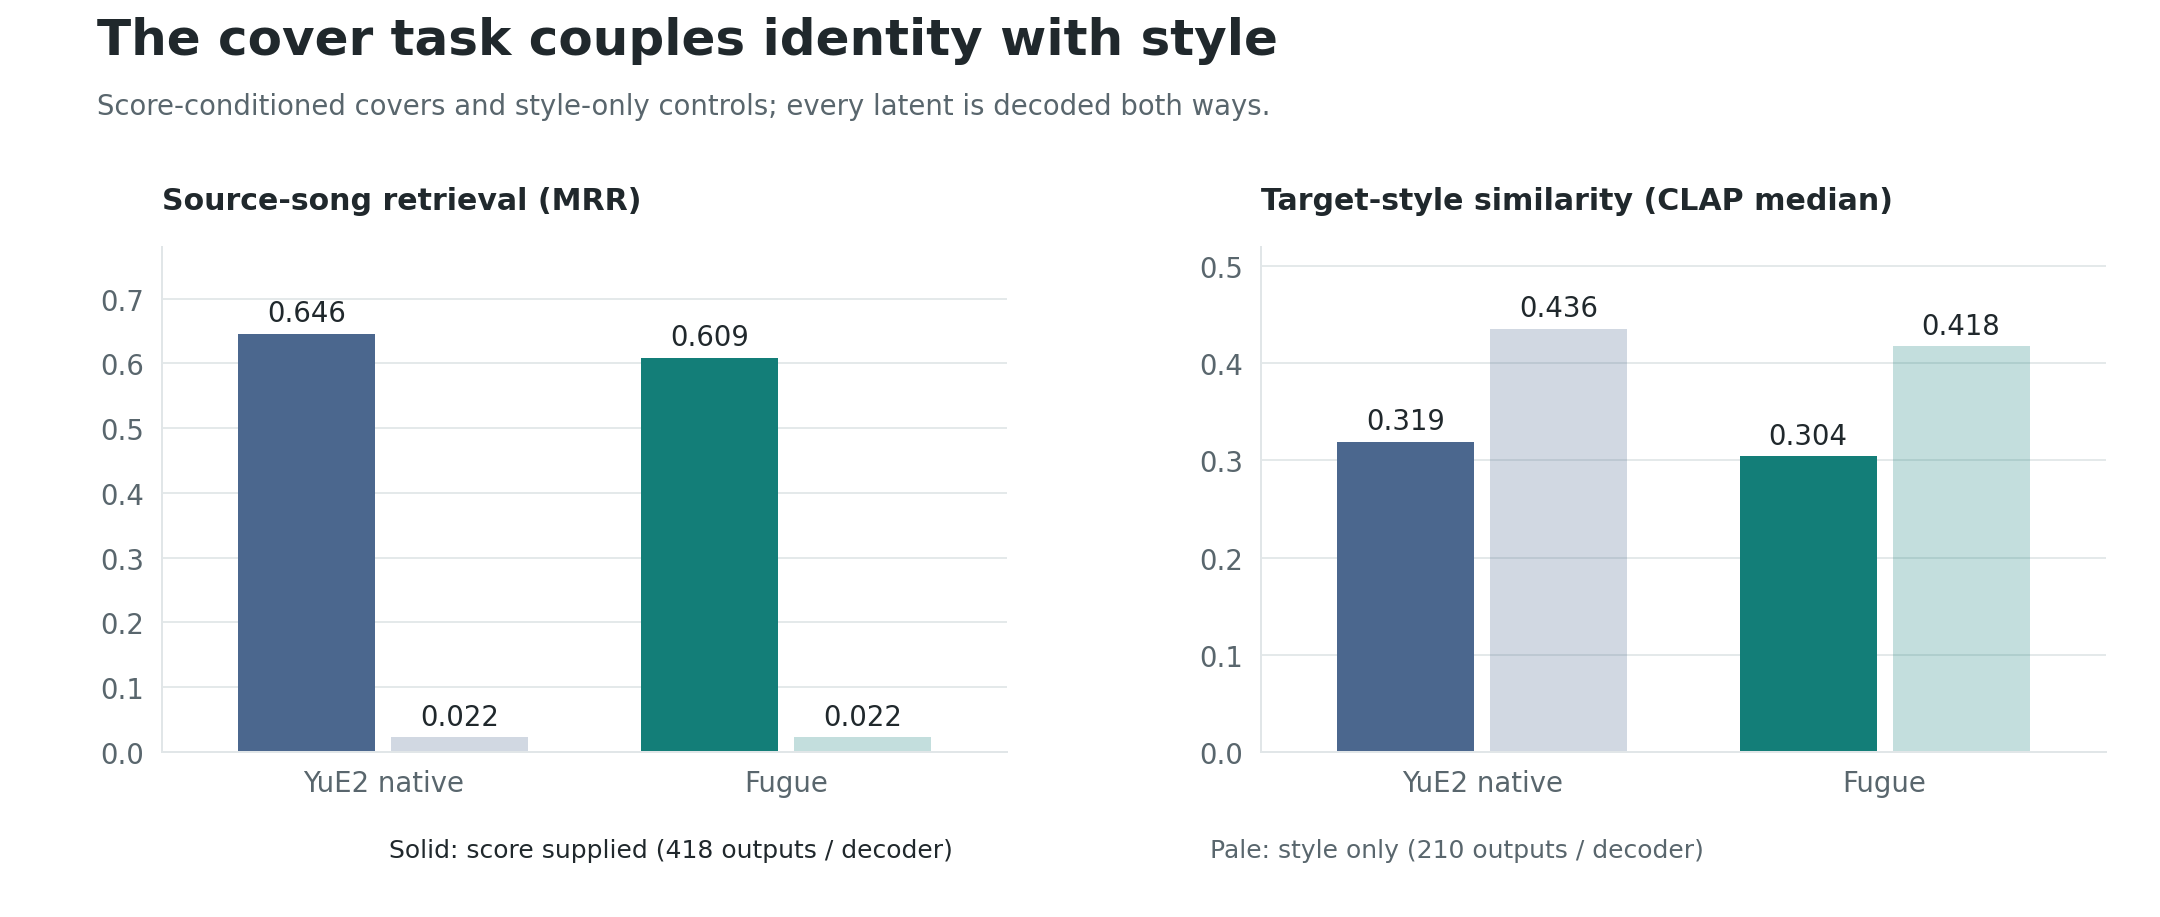
\includegraphics[width=0.96\linewidth]{identity-and-style.png}
    \caption{Identity and style metrics for the two decoders, with and without the source score. Source identity and target style measure different requirements. Removing the score raises the aggregate CLAP median but reduces source retrieval to near-chance performance. The controls use one style per song; score-conditioned evaluation uses two.}
    \label{fig:identity}
\end{figure}

\begin{table}[htbp]
    \centering
    \caption{Identity and style on the local cover benchmark. Both conditions use YuE2 generation and differ in whether the source score is supplied.}
    \label{tab:identity}
    \small
    \begin{tabular}{lrrrrr}
        \toprule
        Input and decoder & $n$ & Hit@1 & Hit@10 & MRR & CLAP median \\
        \midrule
        Source score, YuE2 native & 418 & 0.557 & 0.809 & 0.646 & 0.319 \\
        \textbf{Source score, Fugue} & \textbf{418} & \textbf{0.524} & \textbf{0.775} & \textbf{0.609} & \textbf{0.304} \\
        Style only, YuE2 native & 210 & 0.000 & 0.033 & 0.022 & 0.436 \\
        Style only, Fugue & 210 & 0.000 & 0.033 & 0.022 & 0.418 \\
        \bottomrule
    \end{tabular}
\end{table}

The current version, Fugue v4, retains 94\% of the native decoder's MRR. Its Hit@1 is lower by 3.35 percentage points. Across shared latents, source rank is unchanged in 239 pairs, higher with Fugue in 63, and higher with YuE2 native in 116. The median paired CLAP difference is $-0.019$. These results characterize the current adapter and rendering configuration: much of the source-identification capability is retained, with a measurable retrieval gap.

Several factors may contribute to this gap. Finite adapter regression accuracy can alter song-specific cues, and training on encoded MM3 audio does not eliminate the distribution shift to NAR-generated YuE2 latents. The loss fits \code{c25} rather than directly optimizing source retrieval. Changes in timbre and spatial presentation introduced by the renderer may also change the retrieval embedding. Because the paired decoders receive the same upstream latent, these explanations concern the adapter and rendering path, not different transcription or generation inputs. Their relative contributions have not been isolated in the current version.

Re-transcription DTW medians are 0.470 for YuE2 native and 0.523 for Fugue, computed over 372 and 375 valid outputs. Across the \textbf{372 pairs valid for both decoders}, the median paired difference is 0.000. The corresponding style-only medians are 1.686 and 1.622 over 197 valid outputs each.

\subsection{High-frequency content and stereo image}
\label{sec:acoustic}

The acoustic distinction measured here is increased high-frequency energy and a wider stereo image. These rendering capabilities are inherited primarily from MM3's pretrained DiT-based acoustic path: the DiT synthesizes acoustic latents and the Flow-VAE converts them to stereo waveforms. Fugue contributes the interface that lets YuE2-generated latents drive this path without retraining either component. The paired comparison measures the combined adapter/DiT/vocoder path; it does not isolate the DiT's contribution from the vocoder's.

The release supplies same-latent A/B previews, a source-to-cover comparison in two styles, a vocal example, and five full-length examples: one instrumental piano cover and four vocal covers of two real recordings in two styles each, outside the benchmark catalogue. These examples expose the rendering difference for inspection; they are not a blind-listening evaluation.

\begin{figure}[t]
    \centering
    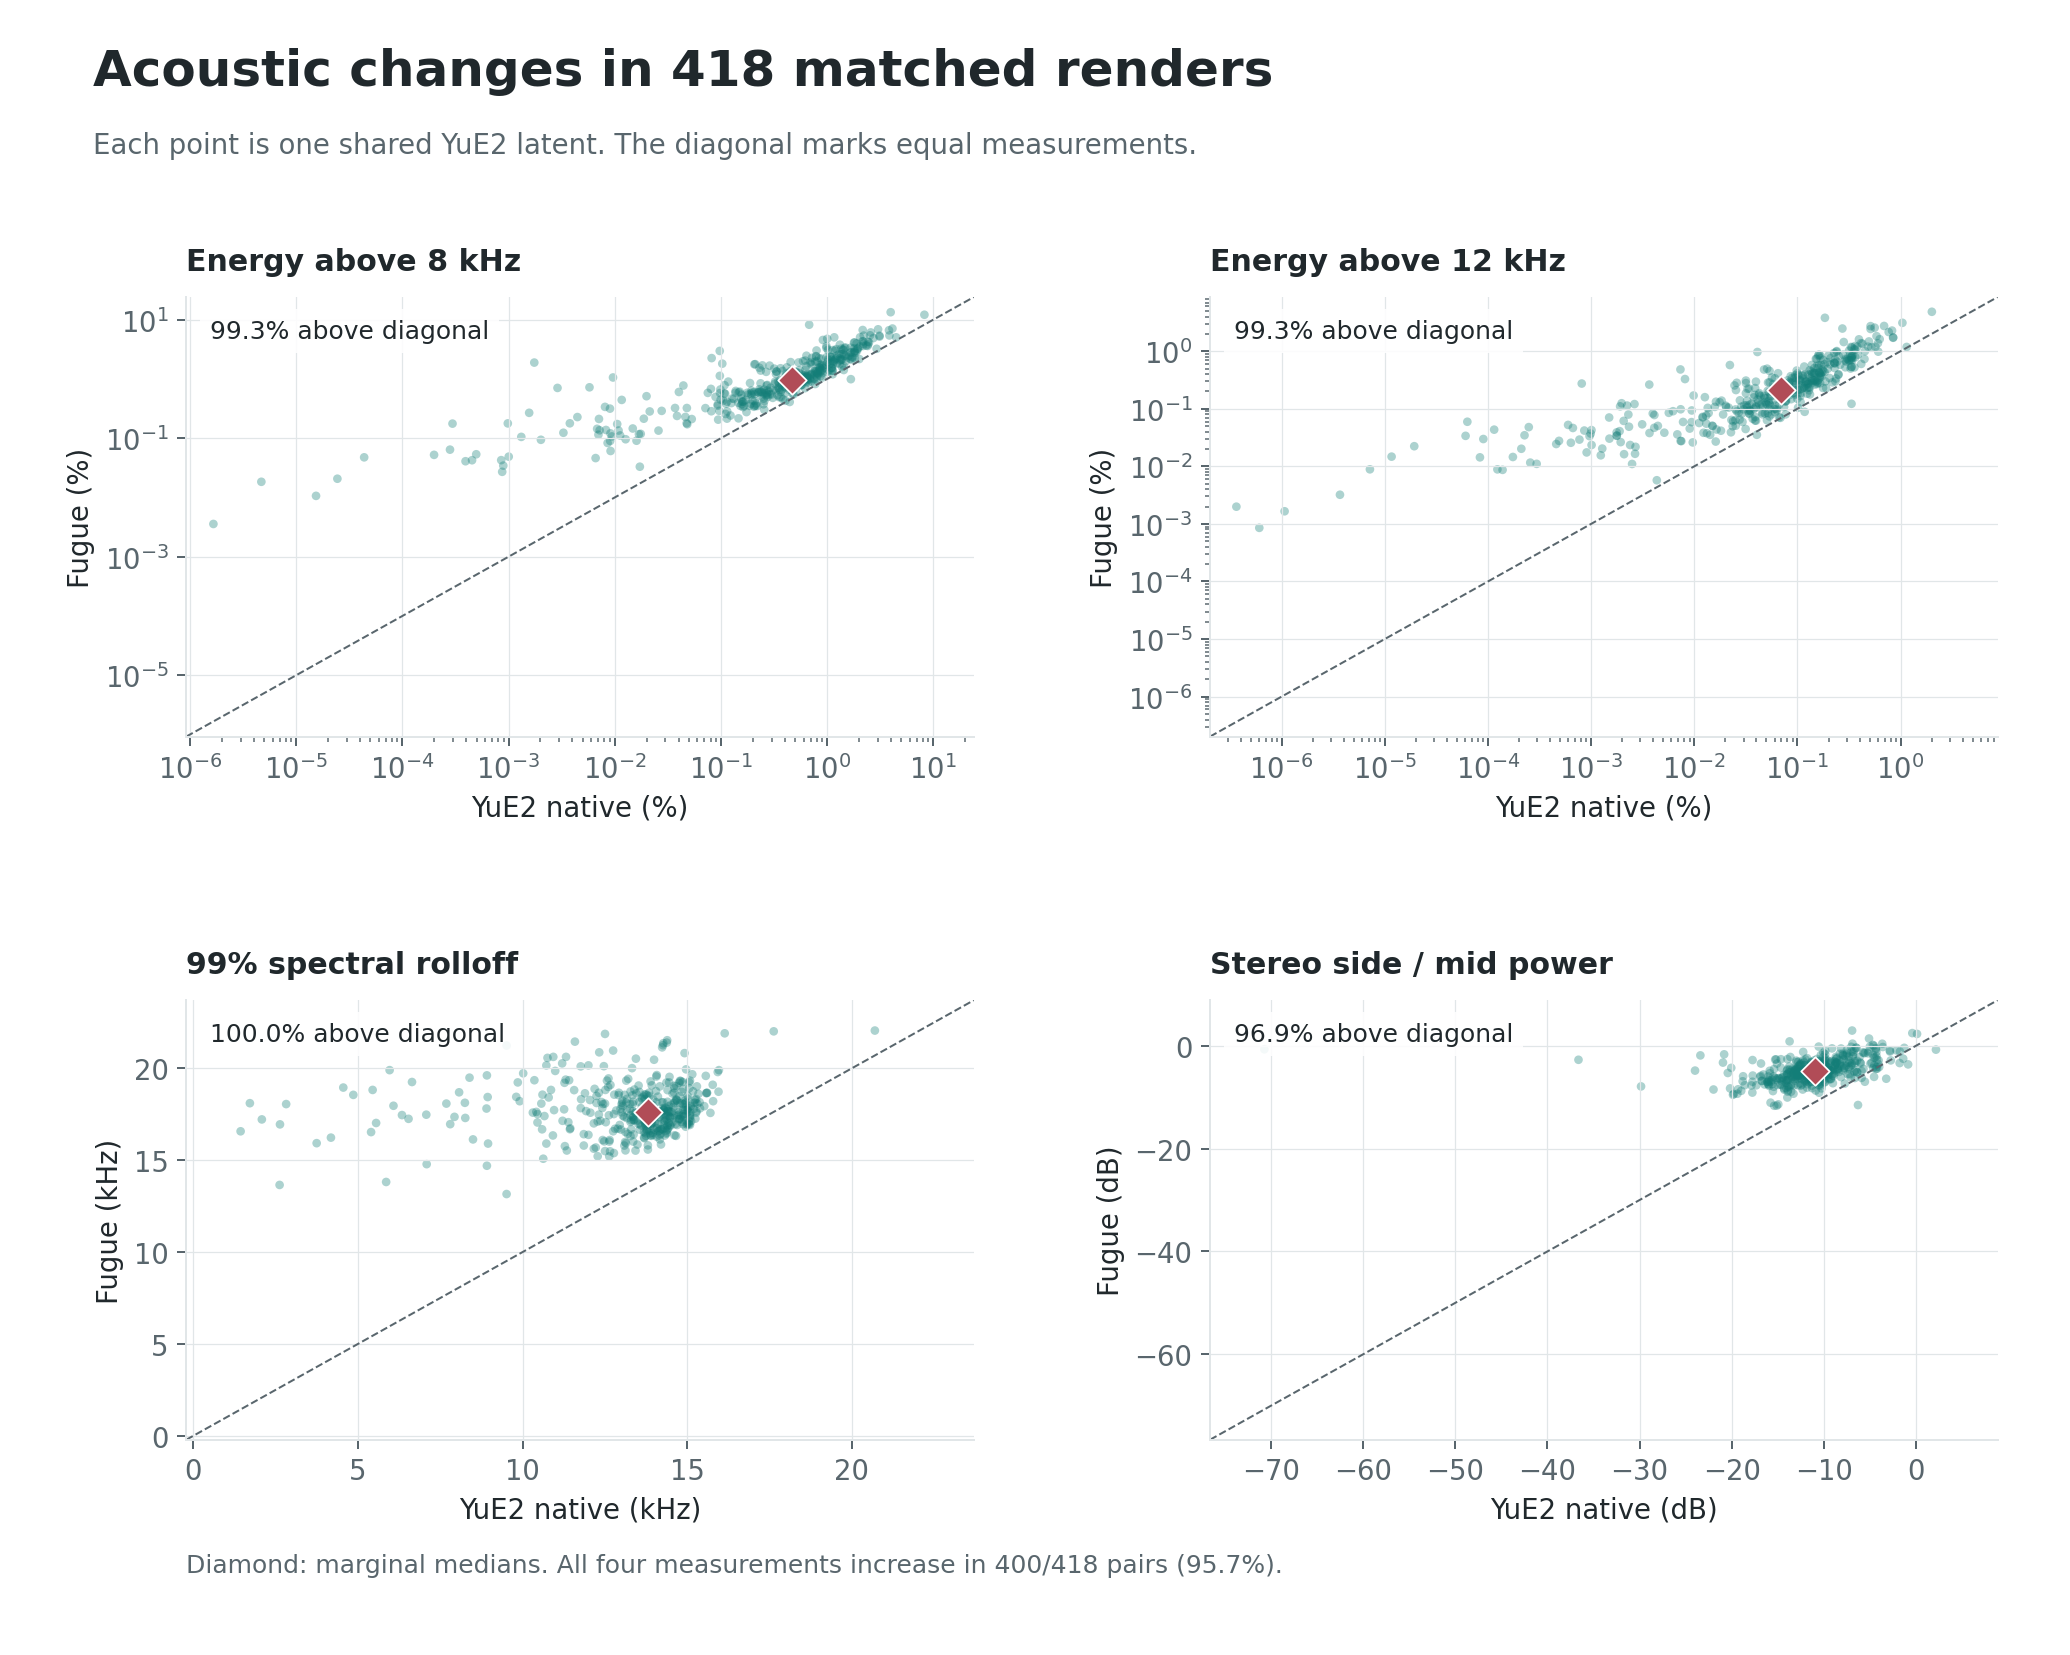
\includegraphics[width=0.96\linewidth]{acoustic-changes.png}
    \caption{Acoustic changes across 418 paired renders. High-band energy axes are logarithmic; rolloff and stereo power use linear axes. The diamond marks the two marginal medians. Values above the diagonal indicate an increase in the plotted measurement, not a perceptual preference vote.}
    \label{fig:acoustic}
\end{figure}

\begin{table}[htbp]
    \centering
    \caption{Spectral and stereo measurements. All four increase simultaneously in 400/418 pairs (95.7\%).}
    \label{tab:acoustic}
    \small
    \begin{tabular}{lrrr}
        \toprule
        Measurement & YuE2 native median & Fugue median & Pairs with an increase \\
        \midrule
        Energy above 8~kHz & 0.466\% & 0.966\% & 415/418 (99.3\%) \\
        Energy above 12~kHz & 0.070\% & 0.209\% & 415/418 (99.3\%) \\
        99\% spectral rolloff & 13.8~kHz & 17.6~kHz & 418/418 (100\%) \\
        Stereo side/mid power & $-10.9$~dB & $-4.8$~dB & 405/418 (96.9\%) \\
        \bottomrule
    \end{tabular}
\end{table}

The median paired differences are $+3.8$~kHz for rolloff and $+6.1$~dB for side/mid power. High-band energy is measured from the mono power spectrum. Rolloff is the median framewise frequency containing 99\% of the cumulative magnitude spectrum. Stereo width is reported as $10\log_{10}\bigl(\operatorname{var}(L-R)/\operatorname{var}(L+R)\bigr)$, with the numerical stabilizers used in \code{eval\_score.py}.

Audiobox-Aesthetics PQ decreases by a median paired 0.278 in the current version. We report this alongside the spectral and stereo measurements: increased high-frequency content and stereo width are not, by themselves, claims of higher perceptual quality. In a separate codec round-trip case study on a real recording, YuE2 VAE achieves SI-SDR 7.7~dB and MM3 Flow-VAE 17.7~dB. This experiment measures codec reconstruction, a distinct question from producing a new arrangement.

\subsection{Full-length covers outside the benchmark}
\label{sec:showcase}

\begin{figure}[t]
    \centering
    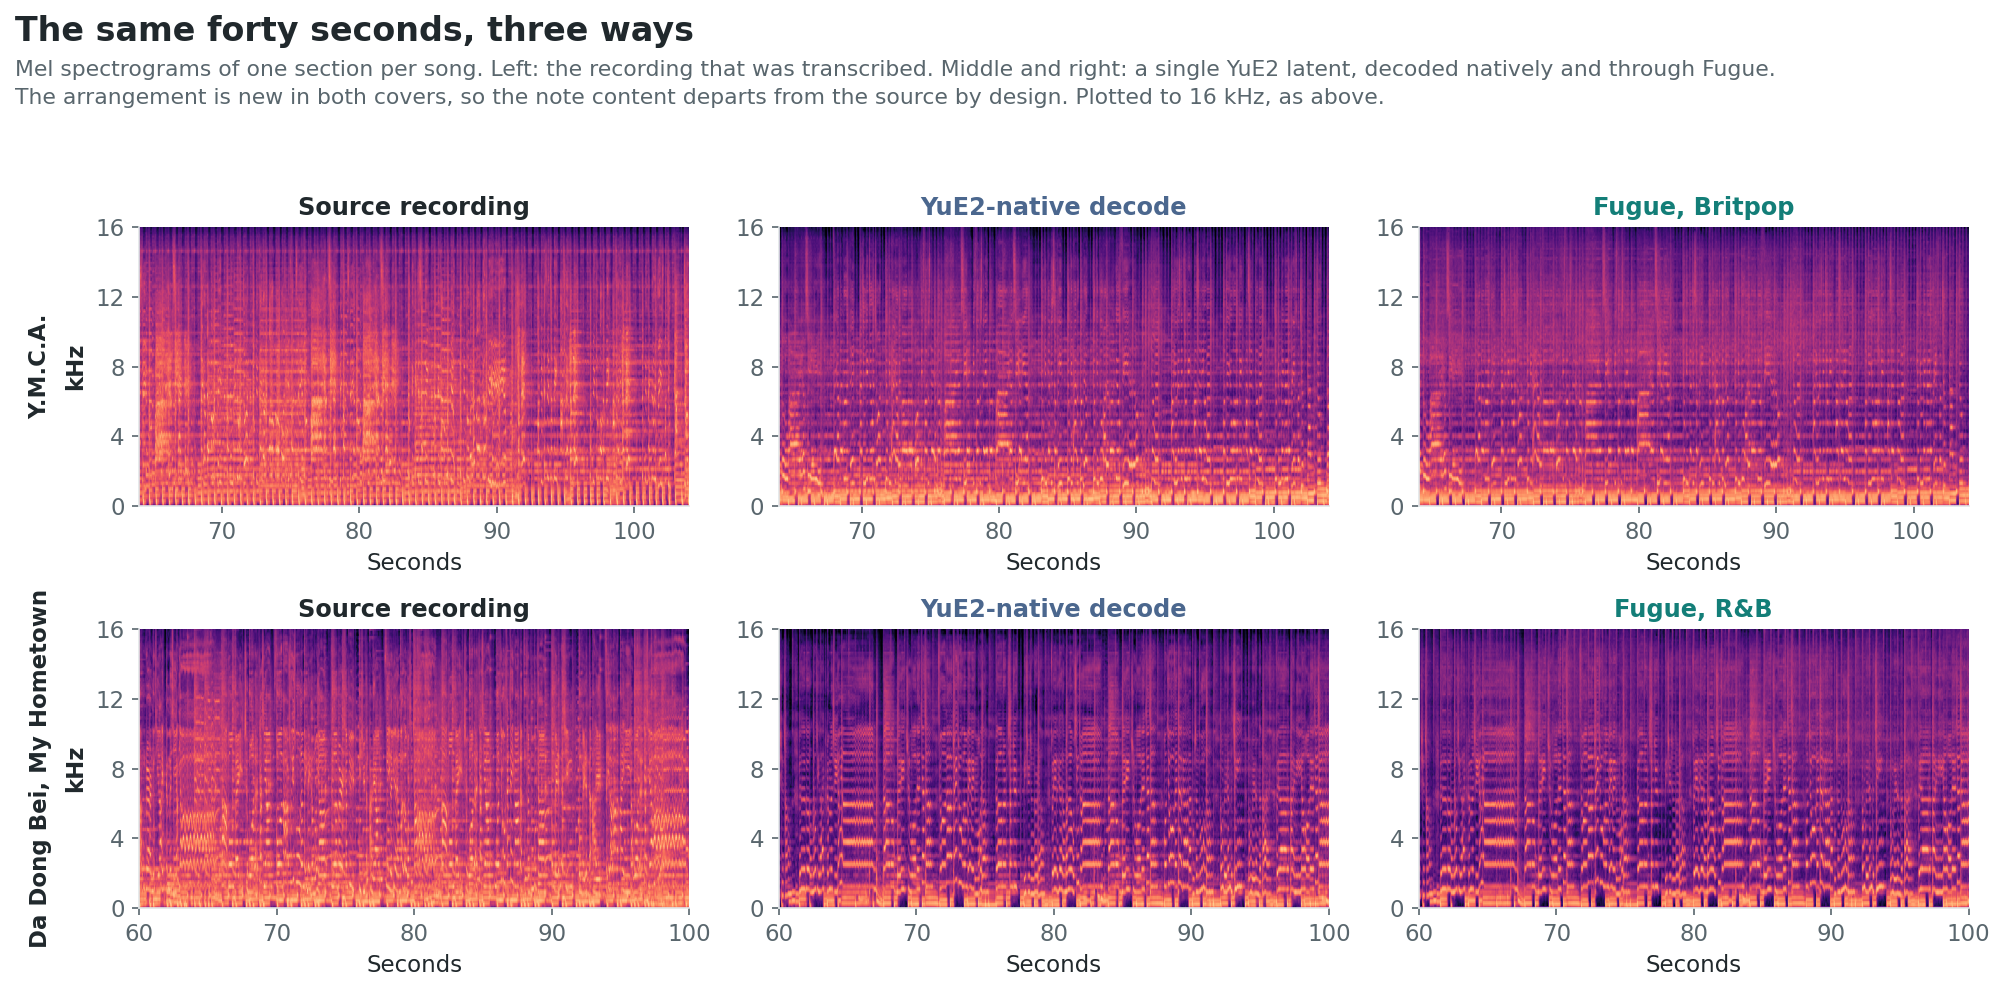
\includegraphics[width=\linewidth]{real-song-covers.png}
    \caption{The same forty seconds of two songs, rendered three ways. Rows are the two source recordings; columns are the source, the YuE2 native decode of the generated latent, and the Fugue render of that same latent. Mel spectrograms are plotted to 16~kHz, which keeps the lossless sources and the MP3 previews comparable above 8~kHz without the MP3 encoder's own lowpass entering the picture.}
    \label{fig:showcase-mel}
\end{figure}

\begin{figure}[t]
    \centering
    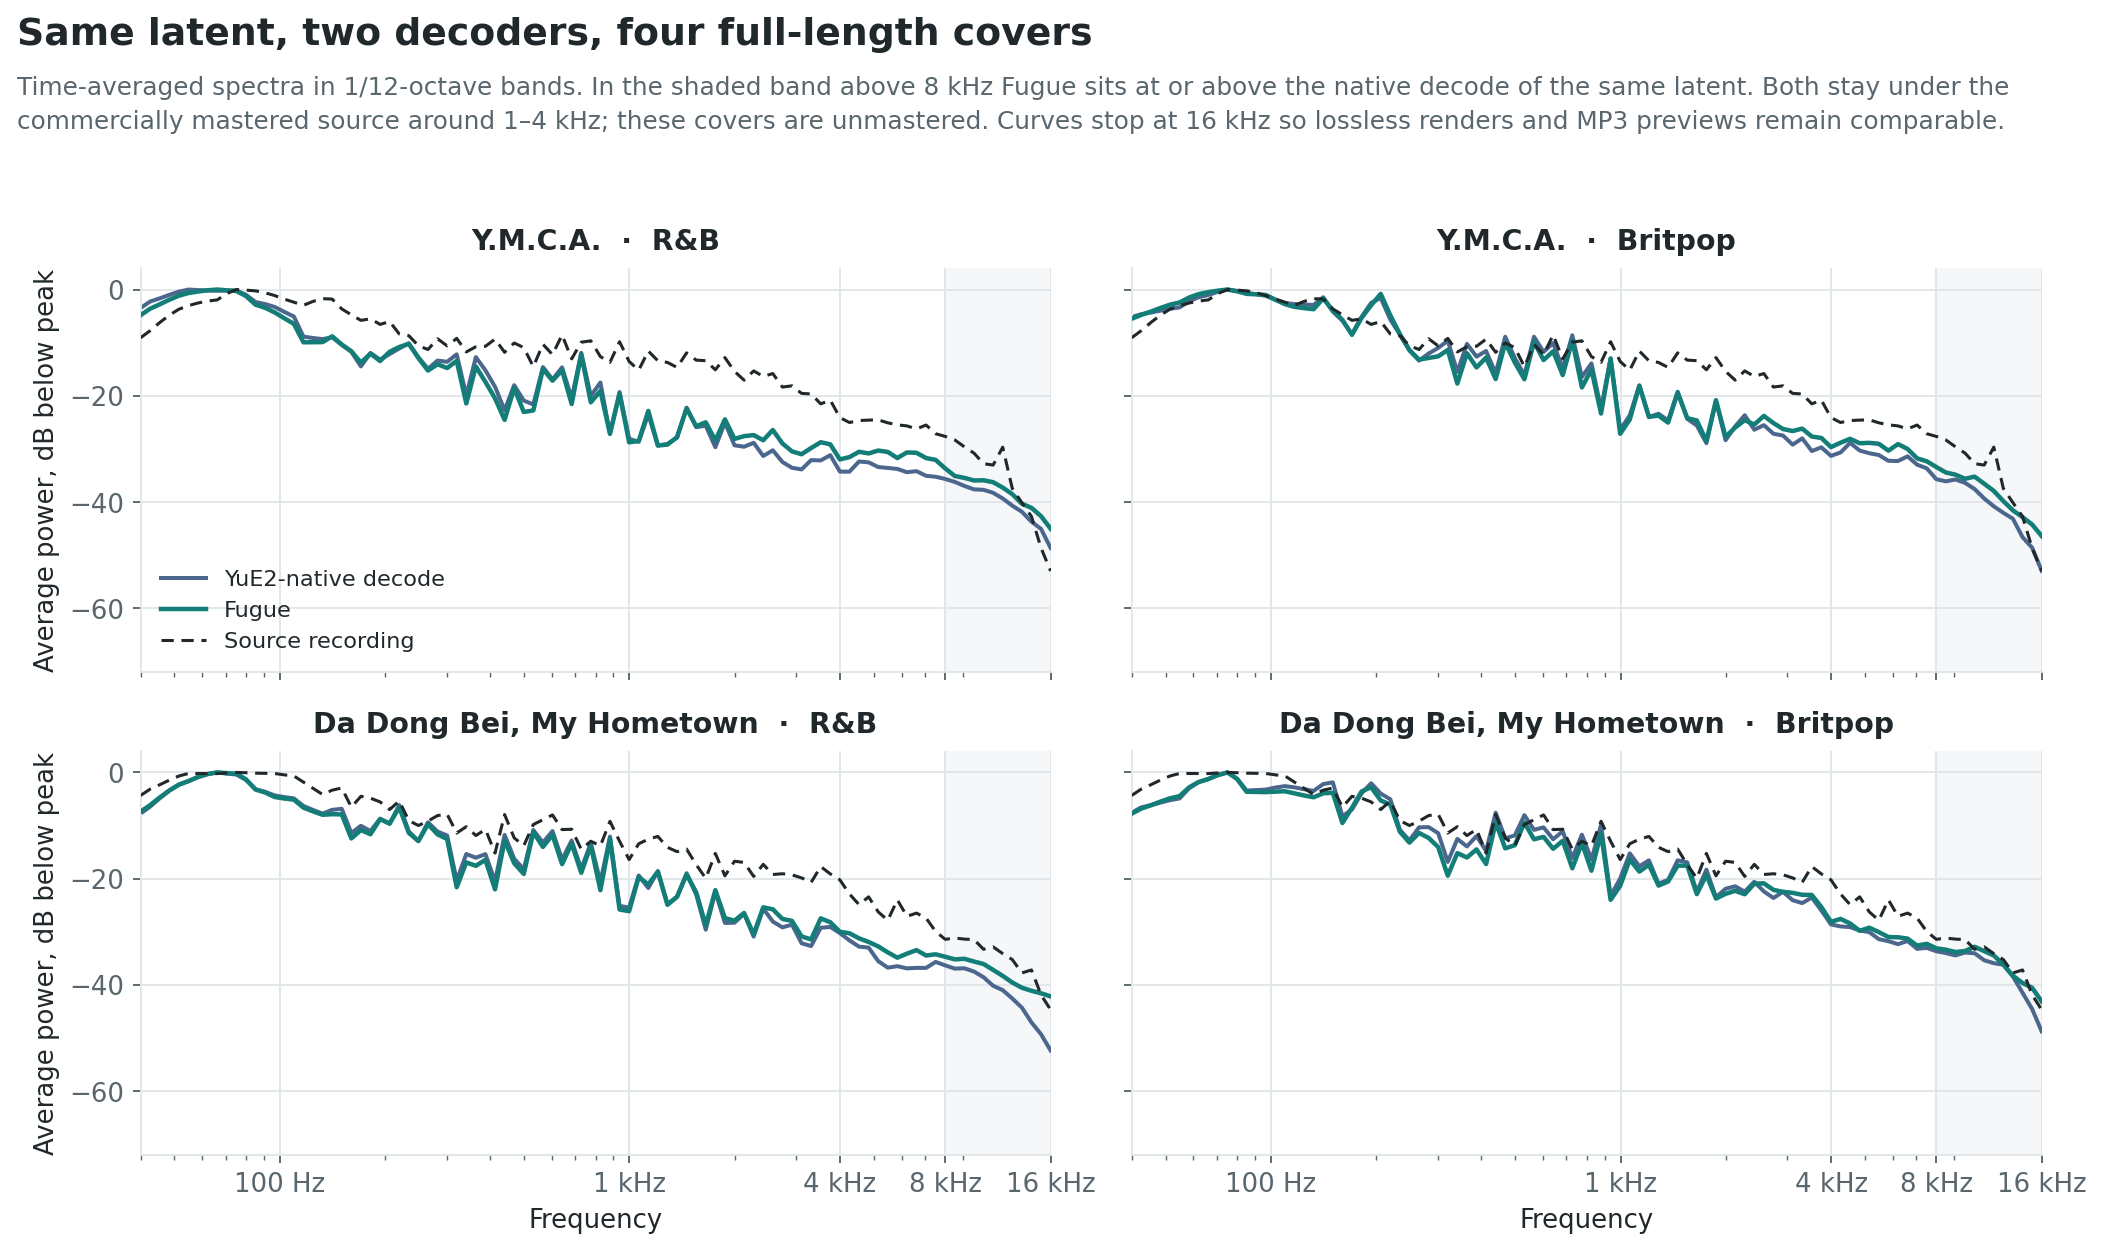
\includegraphics[width=\linewidth]{real-song-spectra.png}
    \caption{Time-averaged spectra of the four full-length covers, pooled into 1/12-octave bands and plotted to 16~kHz. Rows are songs, columns are target styles; each panel overlays the source recording, the YuE2 native decode, and the Fugue render of the same latent. The shaded band marks 8--16~kHz. Fugue sits at or above the native decode of the same latent across these tracks; the gap is a few dB, not an order of magnitude.}
    \label{fig:showcase-spectra}
\end{figure}

The benchmark generations above are instrumental and 60 seconds long. As a separate demonstration, two real recordings outside the benchmark catalogue were covered at full length into two styles each, with vocals. SheetSage2 transcribed each source into a two-voice ABC score with chord annotations, and the lyrics were supplied as text rather than recovered by ASR. Both covers of a song reuse that one score and that one lyric sheet, so the style prompt and the YuE2 seed are the only variables; no BPM appears in the prompts, since the ABC carries its own tempo line. Each track is a single generation with no splicing, 243--284 seconds long, at 171--204 seconds of wall clock on one RTX 4090. Figures~\ref{fig:showcase-mel} and~\ref{fig:showcase-spectra} show these tracks against their sources and against the native decode of the same latent.

These four tracks are a qualitative demonstration and were selected by ear from a larger batch, so they should not be read as an unbiased sample of the acoustic trend in Table~\ref{tab:acoustic}. Measured individually against their sources, they do not all move the same way: the Britpop take of Y.M.C.A.\ carries 0.89\% of its energy above 8~kHz with a 7.6~kHz rolloff, below its own source recording, while the other three sit above theirs. The per-track rendering result is set by what the generator produced, not by a rendering path that raises high-frequency content monotonically. The sources are also commercial masters and the covers have no mastering stage, which accounts for most of the level difference visible between the curves.

% ══════════════════════════════════════════════════════════════
\section{Interface analysis}
% ══════════════════════════════════════════════════════════════

\subsection{What is learned}

\begin{table}[htbp]
    \centering
    \caption{Condition-prediction results from the development runs. Ridge and neural-adapter experiments use different fitting/evaluation subsets; this table is not a controlled scaling comparison. The v4 validation run uses 150 held-out songs. $R^2$ uses the training-channel mean as its reference; it measures condition regression, not cover quality.}
    \label{tab:learned}
    \small
    \begin{tabular}{lrr}
        \toprule
        Adapter or probe & Variance-weighted $R^2$ & Mean channel $R^2$ \\
        \midrule
        Ridge, YuE2 latent with 17-frame context & 0.384 & 0.150 \\
        Ridge, pooled MM3 DAV latent with 17-frame context & 0.201 & 0.086 \\
        v1: 6 layers, width 512, 1,050 training songs & 0.593 & 0.369 \\
        v2: 8 layers, width 768, 10,340 training songs & 0.665 & 0.464 \\
        v3: v2 with variance-weighted loss & 0.672 & 0.462 \\
        \textbf{v4: v3 with input noise, released} & \textbf{0.671} & \textbf{0.461} \\
        \bottomrule
    \end{tabular}
\end{table}

The YuE2 latent is more predictive than the pooled MM3 DAV latent under the tested linear readouts. The Transformer adapters fit the condition better than the ridge baseline.

Input-noise augmentation leaves validation $R^2$ almost unchanged. In the real-song piano case study, v4 reduces re-transcription DTW from v3's 0.434 to 0.369, compared with 0.353 for YuE2 native. On one MM3 reconstruction case, v4 reduces log-mel L1 from v3's 0.787 to 0.740. These cases motivated the release choice; the 209-song benchmark evaluates v4 rather than an all-version ablation.

\subsection{Renderer sensitivity}

\begin{table}[htbp]
    \centering
    \caption{Condition perturbations for one MM3-generated Britpop example. Each row compares its output with the stored original. The separate seed-to-seed distance is 0.698.}
    \label{tab:sensitivity}
    \small
    \begin{tabular}{lr}
        \toprule
        Condition in the 30-second reconstruction case & Log-mel L1 to stored original \\
        \midrule
        Teacher-forced, DiT seed 7 / seed 8 & 0.686 / 0.703 \\
        Added noise, 10\% / 30\% of per-channel variance & 0.697 / 0.729 \\
        Fugue v4 condition predicted from encoded audio & 0.740 \\
        Zero condition & 2.279 \\
        Another song's condition & 5.077 \\
        \bottomrule
    \end{tabular}
\end{table}

This case shows tolerance to moderate unstructured condition error while remaining sensitive to removing or replacing the condition. Learned adapter residuals are structured and may behave differently from Gaussian noise.

The native condition projection and frame rates are documented in Appendix~\ref{app:native}.

\subsection{Infrastructure contribution}
\label{sec:infra}

\paragraph{Training and release pipeline.} Fugue provides the tooling to recover MM3 conditions from saved generation codes, encode the corresponding audio with YuE2, align the two time axes, compute channel statistics, and train the adapter. The inference package loads the adapter weights, normalization statistics, and chunking configuration as one release unit. This packages the learned interface without requiring MM3's LM or depth decoder on the cover-generation path. The research scripts retain laboratory-specific paths; the inference package exposes configurable model locations.

\paragraph{Resident services and orchestration.} The \href{https://github.com/HenryZ838978/fugue/tree/main/services}{service implementation} separates transcription/YuE2 generation from adapter/MM3 rendering, allowing the two dependency environments to remain separate while their models share a GPU. HTTP requests coordinate the stages, and latent files on a shared filesystem carry the intermediate representation. Models remain resident across requests, and the transcription service releases unused CUDA cache after transcription to leave room for the rendering service. The service workflow records requests, intermediate latents, stage timings, and outputs, with separate generation and rendering seeds.

\paragraph{Long-form inference and user interfaces.} The \href{https://github.com/HenryZ838978/fugue/tree/main/fugue}{inference package} implements context-padded adapter windows and connects their output to MM3's native chunked denoising and waveform-stitching procedure. The contribution is making the learned interface work with this existing rendering schedule, not introducing a new DiT or vocoder. A single-process CLI accepts recordings or ABC scores, target styles, and optional lyrics; a service-based CLI and the Arena frontend expose the same cover workflow. The released Arena displays labeled source, YuE2-native, and Fugue outputs for comparison, rather than conducting a blind-listening study.

\paragraph{Paired evaluation and auditability.} The \href{https://github.com/HenryZ838978/fugue/blob/main/research/eval_gen.py}{benchmark driver} shards generation jobs, skips completed items on reruns, and sends each generated latent to both decoders. Per-output records preserve the source/style assignment and generation metadata. The released scoring and figure-generation tools connect these records to the aggregate tables and paired counts. This infrastructure supports inspection and subsequent evaluation extensions without conflating different upstream generations with renderer changes.

\subsection{Runtime and long-form example}

The resident transcription/YuE2 and graft/rendering services occupy approximately 9.8~GB and 4.9~GB on the reference 24~GB GPU. A 30-second cover takes about 50 seconds end to end. A 4:37 piano output was generated with AR, NAR, and acoustic-rendering times of 54, 23, and 118 seconds. These individual runs use resident models; the long example exercises the chunked inference path.

% ══════════════════════════════════════════════════════════════
\section{Discussion: a practical alternative}
% ══════════════════════════════════════════════════════════════

A pretrained generator's default inference pipeline need not be its final interface. Fugue is an instance of \textbf{external adaptation after pretraining}: the learned bridge changes which upstream musical representations can drive a renderer, while the original weights remain fixed. The additional cover capability belongs to the composed system, not to a newly score-trained MM3 backbone.

The intended role is \textbf{a practical alternative for score-conditioned covers with increased high-frequency content and a wider stereo image}. YuE2 supplies score-conditioned musical generation; MM3 supplies the pretrained DiT-based rendering capabilities. Fugue's contribution is the learned connection, its self-generated supervision, and the infrastructure for running and evaluating the composed system. This separates the value of the integrated cover workflow from a claim that Fugue introduced those upstream capabilities.

The engineering question is how to connect these capabilities while keeping the renderer within a useful conditioning regime. Here that leads to a native conditioning target, temporal alignment, channel normalization, and input augmentation. The current version's retrieval gap identifies an interface-level limitation to investigate, rather than establishing an unavoidable cost of frozen-model composition. This report evaluates that version and does not establish an overall ranking against other cover systems.

% ══════════════════════════════════════════════════════════════
\section{Related work}
% ══════════════════════════════════════════════════════════════

\paragraph{Score-conditioned music generation.} YuE2~\cite{yue2} supplies the score-reading and generation capability used by Fugue. MM3~\cite{mm3} supplies the acoustic renderer. The contribution is their composition and its training recipe, isolated by the local paired-decoder study.

\paragraph{Frozen-model composition.} Foley Control~\cite{foleycontrol} connects frozen video embeddings to a frozen text-to-audio DiT through added cross-attention, using video to condition sound. Fugue instead predicts the renderer's existing conditioning representation from another music generator's acoustic latent, with supervision recovered from the renderer's own generations. Freeze-Omni~\cite{freezeomni} likewise shows that speech interfaces can be learned around a frozen language model, using speech/text supervision. Fugue's bridge does not require additional examples of the target original-to-cover transformation.

\paragraph{Representation and readout.} \emph{Where Does the Sound Go?}~\cite{soundgo} finds that acoustic information can remain recoverable in audio-conditioned LLM representations even when downstream answers fail to use it, implicating readout alignment. This motivates distinguishing information available in a representation from behavior expressed by a receiver. Fugue tests a learned interface between frozen modules; its reported results concern this interface, not direct activation steering.

% ══════════════════════════════════════════════════════════════
\section{Current-version limitations and post-release V2}
% ══════════════════════════════════════════════════════════════

The current Fugue v4 benchmark uses a 210-recording gallery, one YuE2 seed, instrumental 60-second generations, and a limited source catalogue. Vocal intelligibility, listener preference, long-form consistency, and generalization across broader genres need dedicated evaluation. The adapter is fitted to MM3-generated audio encodings, while inference uses YuE2-generated latents. Some development examples exhibit renderer-specific timbre shifts. The retrieval and PQ results describe this version's limitations alongside its increased high-frequency content and stereo width.

The present interface controls whole mixed-audio generation through the supplied score and style prompt. It does not guarantee an unchanged selected stem, exact note copying, or independent edits of vocal and instrumental lines.

The initial release makes the system and its current evaluation available first. A post-release \textbf{V2 of this report} is planned to add the following studies; this report revision should not be confused with the earlier v2 adapter run in Table~\ref{tab:learned}:

\begin{enumerate}[leftmargin=2em,itemsep=0.25em]
    \item \textbf{Arena blind listening:} randomized, loudness-matched comparisons with independent listeners, separating audio quality, source-song recognizability, target-style fit, and overall preference.
    \item \textbf{Cover-generation baselines:} comparisons with additional cover systems under matched source songs, target styles, and generation budgets, with expanded retrieval galleries and explicit reporting of failed outputs.
    \item \textbf{Controlled subset ablations:} tests of temporal alignment, input noise, and loss weighting on the same held-out cover subset, using multiple seeds to examine the current retrieval gap and rendering changes.
\end{enumerate}

These are planned extensions after release, not completed experiments or results claimed in the current version.

% ══════════════════════════════════════════════════════════════
\appendix
\section{Direct score-conditioning attempts on MM3}
\label{app:direct}
% ══════════════════════════════════════════════════════════════

Before building the graft, we attempted text-prefix, token-prefix, and in-stream conditioning routes on MM3. The teacher-forcing diagnostic is $d_{\mathrm{spec}} = \mathrm{CE}(\text{other-score}) - \mathrm{CE}(\text{true-score})$: larger positive values indicate that the true score helps predict the audio codes.

\begin{table}[H]
    \centering
    \caption{Direct conditioning attempts on MM3, with the YuE2 control measured on the same diagnostic.}
    \label{tab:direct}
    \footnotesize
    \begin{tabular}{llrr}
        \toprule
        Experiment & Conditioning route & $d_{\mathrm{spec}}$ & Positive paired cases \\
        \midrule
        r1 / r2 & ABC text prefix & approximately 0 & not tabulated \\
        Stage A & Codec-token prefix & approximately 0 & not tabulated \\
        r3 & In-stream and prefix & $+0.0003$ & 26/48 \\
        r4 & Plan loss, condition dropout, tempo retained & $+0.0025$ & 18/24 \\
        YuE2 control & ABC text prefix & $+0.340$ & 24/24 \\
        \bottomrule
    \end{tabular}
\end{table}

In r4, ABC-writing loss fell from 23.1 to 0.49 without a comparable increase in score-conditioned audio prediction. Within the tested settings, learning to produce ABC did not translate into useful score conditioning for audio prediction. These runs motivated reusing YuE2's existing capability.

% ══════════════════════════════════════════════════════════════
\section{Native condition and reproducibility}
\label{app:native}
% ══════════════════════════════════════════════════════════════

MM3's \code{ConditionEncoder} forms a softmax-weighted sum of the LM hidden state and seven RVQ-depth hidden states, applies a learned scalar, and projects with a kernel-3 convolution from 4096 to 2048 channels. The measured mixture coefficients are approximately $[0.906, 0.013, 0.013, 0.013, 0.014, 0.014, 0.014, 0.014]$, and the scalar is 0.0685. Projection and normalization elsewhere in the model prevent interpreting that scalar alone as the strength of conditioning.

The condition rate is $24000/960 = 25$~Hz; the acoustic latent rate is $44100/512 = 86.1328125$~Hz. The nominal upsampling ratio is $441/128 = 3.4453125$, with integer output lengths per chunk. These are representation frame rates, not bounds on waveform frequency content.

The released \href{https://github.com/HenryZ838978/fugue/blob/main/research/eval_summary.json}{summary} and \href{https://github.com/HenryZ838978/fugue/blob/main/research/eval_per_item.json}{per-output records} support Tables~\ref{tab:identity}--\ref{tab:acoustic} and Figures~\ref{fig:identity}--\ref{fig:acoustic}. \href{https://github.com/HenryZ838978/fugue/blob/main/paper/figures/render_figures.py}{The figure script} validates the summary against those records, derives the paired counts, and exports SVG and PNG; \href{https://github.com/HenryZ838978/fugue/blob/main/paper/figures/render_showcase.py}{a second script} renders Figures~\ref{fig:showcase-mel} and~\ref{fig:showcase-spectra} from the showcase audio and its stored curves. The development analyses in Tables~\ref{tab:learned}--\ref{tab:sensitivity} are documented in the \href{https://github.com/HenryZ838978/fugue/blob/main/research/SCION.md}{historical lab notebook}. The \href{https://github.com/HenryZ838978/fugue/blob/main/samples/README.md}{sample index} identifies the preview audio and generation settings.

% ══════════════════════════════════════════════════════════════
\begin{thebibliography}{9}
\small\raggedright\setlength{\itemsep}{2pt}
\bibitem{yue2} M-A-P. \emph{YuE2-3B}. Model card and inference implementation, 2026. \code{m-a-p/YuE2-3B} on Hugging Face.

\bibitem{mm3} MiniMax. \emph{MiniMax-Music3}. Model release, 2026. \code{MiniMaxAI/MiniMax-Music3} on Hugging Face.

\bibitem{discogsvi} R. Oguz Araz, Xavier Serra, and Dmitry Bogdanov. \emph{Discogs-VI: A Musical Version Identification Dataset Based on Public Editorial Metadata}. ISMIR, 2024. arXiv:2410.17400.

\bibitem{foleycontrol} Ciara Rowles et al. \emph{Foley Control: Aligning a Frozen Latent Text-to-Audio Model to Video}. 2025. arXiv:2510.21581.

\bibitem{freezeomni} Xiong Wang et al. \emph{Freeze-Omni: A Smart and Low Latency Speech-to-speech Dialogue Model with Frozen LLM}. 2024. arXiv:2411.00774.

\bibitem{soundgo} Song-ha Jo et al. \emph{Where Does the Sound Go? Tracing Acoustic Information Loss in Audio-Conditioned LLMs}. 2026. arXiv:2609.05871.
\end{thebibliography}

\end{document}
